\documentclass[border=2pt]{standalone}
\usepackage{tikz}
\usetikzlibrary{automata,shapes.geometric}

\begin{document}
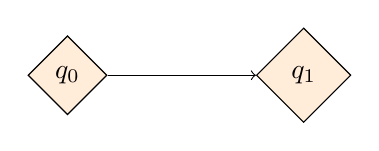
\begin{tikzpicture}[every state/.style={fill=orange!15}]
  \node[state,initial by diamond] (single) at (0,0) {$q_0$};
  \node[state,initial by diamond,minimum size=12mm] (large) at (3,0) {$q_1$};
  \draw[->] (single) -- (large);
\end{tikzpicture}
\end{document}
